\documentclass[preprint]{sig-alternate-10pt}

\usepackage{alltt}
\usepackage{balance}
\usepackage[hyphens]{url}

\usepackage{etoolbox}
\usepackage{graphicx}
\usepackage[font=small,labelfont=bf]{caption}
\apptocmd{\thebibliography}{\scriptsize}{}{}
\usepackage[utf8]{inputenc}

\usepackage[paperwidth=8.5in,paperheight=11in,margin=1in]{geometry}

\newcommand{\para}[1]{\vspace{2mm}\noindent\textbf{#1}}
\newcommand{\name}[1]{\textsf{\small #1}}

\begin{document}

\title{Dagstuhl Seminar on Big Stream Processing}

\iffalse
\numberofauthors{5}
\newcommand*{\emailn}[1]{\textsf{\normalsize #1}}

\author{
\alignauthor
Sherif Sakr\\
  \affaddr{KSAU-HS and UNSW}
  \emailn{ssakr@cse.unsw.edu.au}
\alignauthor
Tilmann Rabl\\
  \affaddr{TU Berlin, Germany}\\
  \emailn{rabl@tu-berlin.de}
\alignauthor
Martin Hirzel\\
  \affaddr{IBM Research AI, USA}\\
  \emailn{hirzel@us.ibm.com}
\and
\alignauthor
Paris Carbone\\
  \affaddr{KTH EECS, Sweden}\\
  \emailn{parisc@kth.se}
\and
\alignauthor
Martin Strohbach\\
  \affaddr{AGT International, Germany}\\
  \emailn{mstrohbach@agtinternational.com}}
\fi

\numberofauthors{1}
\author{\sffamily\hspace*{-4.2mm}\begin{tabular}{c@{\hspace*{2mm}}c@{\hspace*{2mm}}c@{\hspace*{2mm}}c@{\hspace*{2mm}}c}
  \large Sherif Sakr
& \large Tilmann Rabl
& \large Martin Hirzel
& \large Paris Carbone
& \large Martin Strohbach\\
  \normalsize KSAU-HS \& UNSW
& \normalsize TU Berlin, Germany
& \normalsize IBM Research AI
& \normalsize KTH EECS, Sweden
& \normalsize AGT International, Germany\\
  \small ssakr@cse.unsw.edu.au
& \small rabl@tu-berlin.de
& \small hirzel@us.ibm.com
& \small parisc@kth.se
& \small mstrohbach@agtinternational.com
\end{tabular}}

\maketitle

\begin{abstract}
Stream processing can make sense of big data in real time as it is
being produced. This paper reports findings from a 2017 seminar on big
stream processing, focusing on applications, systems, and languages.
\end{abstract}

\section{Overview}\label{sec:overview}

As the world gets more instrumented and connected, we are witnessing a
flood of digital data that is getting generated, at high velocity,
from different hardware (e.g., sensors) or software in the form of
streams of data. Examples of this phenomenon are crucial for several
applications and domains including financial markets, surveillance
systems, manufacturing, smart cities, and scalable monitoring
infrastructure. In these applications and domains, there is a crucial
requirement to collect, process, and analyze big streams of data in
order to extract valuable information, to discover new insights in
real-time, and to detect emerging patterns and outliers. Since 2011
alone, several systems (e.g.,
Storm~\cite{toshniwal_et_al_2014},
Apache Apex\footnote{\url{https://apex.apache.org/}},
Spark Streaming~\cite{zaharia_et_al_2013},
Apache Flink~\cite{carbone_et_al_2015}, and
Heron~\cite{kulkarni_et_al_2015}) have
been introduced to tackle the real-time processing of big streaming
data. However, there are several challenges and open problems that
need to be addressed in order improve the state-of-the-art in this
domain and to achieve wide adoption of big stream processing systems
by large number of users and enterprises~\cite{sakr2016big}.

This report is based on a five-day workshop on ``\emph{Big Stream
  Processing Systems}'' that took place at Schloss Dagstuhl in Germany
from 29~October to 3~November 2017\footnote{\url{http://www.dagstuhl.de/en/program/calendar/semhp/?semnr=17441}}. The workshop was attended by 29
researchers from from 13 countries. Participants came from different
communities including systems, query languages, benchmarking, stream
mining and semantic stream processing. A major benefit of this
workshop was the opportunity for scholars from different communities
to get exposure to each other and get freely engaged in direct and
interactive discussions. The seminar program consisted of tutorials on
the main topics of the workshop, lightning talks by participants on
their research, and two working groups dedicated to deeply
investigating selected topics. The first group focused on applications
and system of big stream processing while the second group focused on
analyzing the state-of-the-art of stream processing languages. This
report presents highlights from the workshop program.

\section{Tutorials}
The tutorials of the seminar aimed at sharing knowledge between
attendees from different communities, thus offering insights and
perspectives that enriched the group discussions. This section gives
an overview of the material presented at tutorials.

\subsection{IoT Stream Processing Applications}
This tutorial analyzed IoT applications from two domains: sports and entertainment as well as Industry 4.0. The application examples are based on commercial deployments using AGT International's\footnote{\url{http://www.agtinternational.com}} Internet of Things Analytics (IoTA) platform.

\iffalse
In sports and entertainment we described specific characteristics of IoT streaming applications and the associated challenge of choosing an appropriate streaming infrastructure. In the Industry 4.0 domain we showed how stream processing applications can be benchmarked using the HOBBIT benchmarking platform.
\fi

\para{Sports and Entertainment}
The example applications of this domain provide real-time narratives about highlights that are happening during a live event. This way, it is not necessary to watch the whole event, but one can be notified in real-time about such highlights based on insights derived from sensor data. For instance, in \emph{basketball}, sensors that have been successfully used in commercial deployments\footnote{\url{https://t.co/ZkQjQwXw13}} include smart shirts worn by players, microphones deployed to monitor the audience,  cameras and wristbands. Data from these sensors in combination with play-by-play data can be used to recognize behaviour, emotions, activities, actions, pressure and other physical aspects about the game. These insights are related to players, teams, fans and family that are preferably provided as semantic data streams. Semantic data access decouples applications from data providers and enables domain experts to better work with the data, e.g. for generating content and distributing it via social media.
%Figure Basketball ?

Another example is \emph{mixed martial arts}\footnote{\url{https://youtu.be/vataVq9gY_o}} in which sensors such as cameras, smart floors and sensors embedded in fighters' gloves\footnote{\url{http://bit.ly/2D4lCqD}} are used in order to determine a range of insights including punch strength and stress levels of each fighter (Figure~\ref{FIG:FightStreams}). In this example, it is important that insights can be delivered in real-time without noticeable delay compared to a broadcast of the fight.

\begin{figure}[t]
\centering
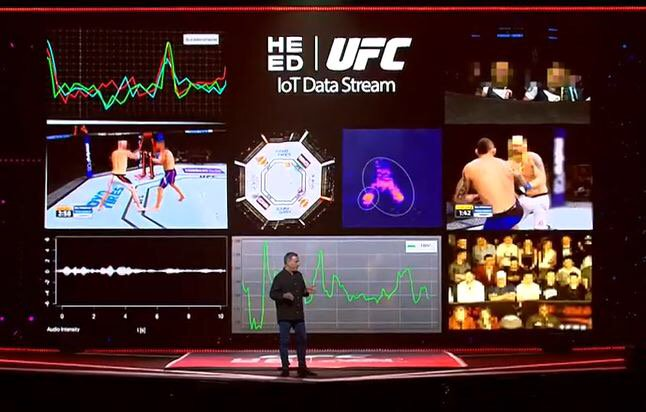
\includegraphics[scale=0.142]{pictures/DP6L8S9XkAYFMCw.jpg}
\captionof{figure}{Sample IoT data streams in mixed martial arts.}
\label{FIG:FightStreams}
\end{figure}

In \emph{professional bull riding}, sensors are attached to riders and bulls and used in order to quantify the bull's and rider's performance\footnote{\url{http://bit.ly/2CXpc2g}}. As this information is among others used for automatic scoring, it is of particular importance that analytic results are available as soon as the ride is finished. Similarly, a range of wearable sensors are used for creating event highlights for participants at \emph{mass sport events} such as the Color Run\footnote{\url{https://thecolorrun.com/}}. In the \textsf{CPaaS.io} project\footnote{\url{http://www.cpaas.io}}, an application has been developed to use action cameras and fitness bands to automatically detect event highlights based on the the runner's activity, emotions, dance energy levels, and many more metrics. In this application, real-time aspects include scenarios in which event highlights are being directly sent to friends of the participants.

\para{Industry 4.0}
For this domain, the tutorial presented applications related to \emph{predicting energy peaks} and \emph{predictive maintenance}. In principle, predicting energy peaks can help in reducing energy costs as electricity bills of industrial consumers contain a pricing component that incurs higher charges for higher peaks of electrical load. For a small to medium enterprise, avoiding such peak load events can lead to significant savings\footnote{\url{http://bit.ly/2DjhvUh}}. This can be achieved by predicting expected peaks e.g. up to 30 minutes ahead of time and taking precautious measures such as temporarily switching off high energy consumers such as air conditioning.

For \emph{predictive maintenance}, the tutorial presented an application for detecting anomalous machine states in order to reduce maintenance costs. For instance, in injection molding machines a sudden high energy consumption may indicate that an injection nozzle is jammed and checking the machine may avoid further damage. The tutorial reported about the DEBS Grand Challenge 2017~\cite{gulisano_et_al_2017} that has been designed to objectively measure some of these requirements using pre-defined machine learning algorithms and RDF streaming data. The main KPI for the challenge was latency. The original data set has been provided by \textsf{Weidmüller}\footnote{\url{http://www.weidmueller.de}}. For reasons of confidentiality, the organizers provided a mimicked data set\footnote{\url{https://hobbit.iminds.be/dataset/weidmuller}}. The systems under test were evaluated using the \textsf{HOBBIT} benchmarking platform\footnote{\url{http://bit.ly/2muMNkY}} that ensured the objectivity of quantifying the performance of distributed stream processing pipelines. \iffalse As we used a pre-defined algorithm for detecting anomalies, we expected full correctness from all systems and compared latency and also measured throughput.\fi Overall, 7 out of 14 participating teams in the challenge passed the correctness test. The fastest system~\cite{amariei_et_al_2017} achieved an average latency of about 39ms. The DEBS Grand Challenge 2017 benchmark is openly available as part of the HOBBIT platform.

%Systems under test had to correctly answer a pre-defined query that describes an anomaly in the expected machine states. The task involved to find k cluster centers in a sliding window in order to identify the machine states. As a next step, it was required to build a Markov model over the sliding window and use it to determine the probability of the last N state transitions. Finally, if the probability is below a given threshold the system under test had to report an anomaly. Machines could dynamically leave and join.




%\subsubsection{Choosing the Streaming Infrastructure}
%When choosing a streaming infrastructure fulfilling the requirements of the above application scenarios, we face the following challenges

%\begin{itemize}
%  \item Lack of standardized query language for streaming applications
 % \item Flexibility for Programming Languages
 % \item Low Latencies and short-lived stream processing pipelines
% semantic mapping has been briefly mentioned in the sports and entertainment app
%  \item Semantic mapping
%\end{itemize}

%While in the database world there are standardized query languages such as SQL and SPARQL, there is still no standard stream processing language (see Section \ref{sec:tut_lang}). As a consequence streaming applications are very closely coupled to the underlying stream processing system making the choice of the infrastructure a critical one.

%When considering the applications above, it becomes apparent that the implementation of a variety of analytical modules are required. However, there is a discrepancy between the tools and programming languages typically used by data scientist (Python, Julia, C/C++, R, Matlab, etc.) and the mainly JVM based languages (Java and Scala) that are supported in common stream systems as described in section \ref{sec:tut_systems}. Although python is increasingly supported in these systems, resource management of JVM external languages is badly supported. However, such external resources may be considerable, e.g. if machine learning models are involved. And languages other than Python are not directly supported at all.

%Finally, IoT streaming applications as described above require low latency processing pipelines rather than supporting an extremely high number of throughput. In addition there may be a large number of short-lived rather than a few long-lived processing pipelines. In typical settings there may thousands of sensor streams connected to the system and a multitude of analytical results created from all the streams. However, not all streams are equally important at all times. For instance, in a sports tournament there may be a couple of standard pipelines being set up for the duration of the tournament, but many more smaller pipelines are set up for the duration of a single match, half or quarter. Some pipelines are only set up, based on ad-hoc queries. For the shorter-lived pipelines it is extremely important that the pipeline including its analytics module can be set up extremely fast, i.e. below one second, including tasks such as the deployment and resource allocation of analytics module and the models they use. To our knowledge virtually all existing and mature frameworks focus on high throughput and long lived processing pipelines and thus do not fully support these requirements.


%!TEX root = main.tex

\subsection{Big Stream Processing Systems}
\label{sec:tut_systems}
%\begin{alltt}TODO\scriptsize 0.75/1 pages
%\end{alltt}

This tutorial started by identifying the most differentiating characteristic of scalable data stream processing systems, which is the notion of data as a continuous, possibly infinite resource instead of ``facts and statistics organized and collected together for future reference or analysis''\footnote{Definition of ``data'' according to Google Dictionary}. In fact, data stream processing systems broaden their context from retrospective data analysis to continuous, unbounded processing coupled with scalable and persistent application state.  Various forms of stream processing have been employed in the past within their respective domains, such as network-centric processing on byte streams, functional (e.g., monads) and actor programming, complex event processing, and database materialized views. Besides, \emph{stream management} has been an active research field for decades~\cite{abadi2003aurora,arasu2004stream,chandrasekaran2003telegraphcq}. Nonetheless, several of these ideas have  only just recently been put together in a consistent manner to compose a stack  centered around the notion of data as an unbounded partitioned stream of records (Figure~\ref{fig:streamstack}). Most importantly, stream processing did not restrict but complemented existing scalable processing models (e.g., MapReduce \cite{dean2008mapreduce}) with persistent partitioned state, time domains, and flexible scoping using stream windows. The general programming stack  addresses storage, compute, and domain-specific library support.

\begin{figure}[t]
\centering
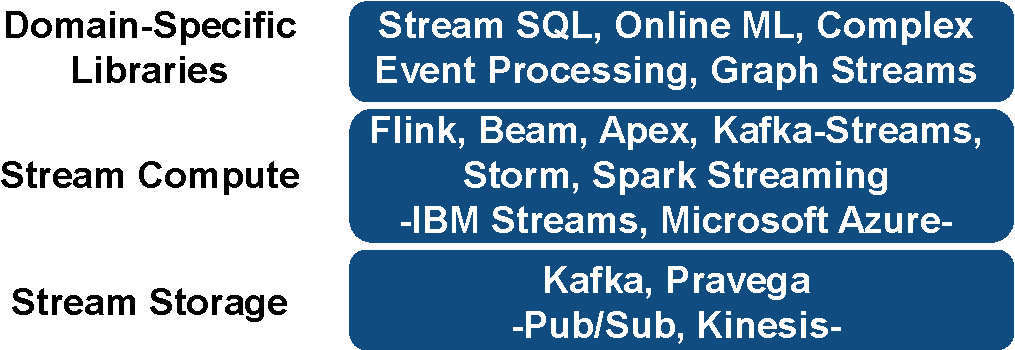
\includegraphics[width=0.4 \textwidth]{pictures/streamstack.pdf}
\caption{The Stack of Scalable Stream Processing}
\label{fig:streamstack}
\end{figure}

\para{Stream Storage.} Data dissemination from consumers to producers is a problem that has been revisited multiple times with different assumptions and needs in mind. In the context of data streaming, direct communication (e.g., TCP channels) was not an option despite low-latency requirements, since it required application ingestion to be actively in sync with data creation while also lacking the transparency and durability properties that are the norm in today's cloud computing ecosystem. Furthermore, message brokers (e.g., \textsf{\small RabbitMQ}, \textsf{\small JMS}) were insufficient for the needs of supporting multiple applications and configurations (i.e., task parallelism). Thus, a class of open-source stream storage systems based on \emph{partitioned replicated logs} was introduced, led by \textsf{\small Apache Kafka}~\cite{kreps2011kafka} and more recently \textsf{\small Pravega}\footnote{\url{http://pravega.io/}} as well as proprietary cloud services such as \textsf{\small Amazon Kinesis}\footnote{\url{https://aws.amazon.com/kinesis/}}. Partitioned replicated logs provide high sequential read and write throughput by exploiting copy-on-write and strict data-parallel access by distinct consumers. Furthermore, they bookkeep data access (offset-based) for the purposes of data reprocessing, reconfiguration, and roll-backs, among others. Finally, more effort has been devoted to supporting transactional logging and repartitioning, allowing for seamless integration with modern stream compute systems.

\para{Stream Compute.} We further divide compute into \emph{programming models} and \emph{runtime engines}. In terms of programming model support, there has been a shift from purely event-based, compositional models (e.g., \textsf{\small Apache Storm} \cite{toshniwal_et_al_2014}) to more declarative representations~\cite{carbone_et_al_2015,akidau2015dataflow,zaharia_et_al_2013}. Currently, most standard APIs are fluid, functional, and allow declaring relational transformations (e.g., joins, filters etc.) while providing first-class support for persistent partitioned state, stream windows, and event-time prog\-ress using watermarks. The latter allowed application logic to incorporate timers that operate consistently on different time domains (e.g., origin-time), thus allowing out-of-order processing~\cite{li2008out},  a concept popularized by Google \cite{millwheel,akidau2015dataflow}.

With respect to runtime engines, we observe certain converging commonalities such as a dataflow execution model, explicit locally embedded state (using log-compaction trees \cite{CUSTOM:web/rocksdb}) and asynchronous state snapshotting for fault tolerance and reconfiguration support \cite{state2017carbone,jacques2016consistent}. Apache Spark \cite{zaharia_et_al_2013}, as a special case, emulates data streaming by slicing computation into recurring batch jobs, yet, it currently makes use of locally embedded state and there are plans to adopt a continuous processing runtime as well for the purposes of low-latency data streaming.

\iffalse
\para{Domain-Specific Libraries.} A concluding discussion in this tutorial addressed the prospects of standardizing domain-specific libraries such as Stream SQL, CEP, Online Machine Learning and User-Defined Windows \cite{carbone2015cutty} as well as system runtime concepts that are indirectly exposed to the user such as state snapshots \cite{state2017carbone}. Several of these initiatives can already be observed in the effort of Apache Beam \cite{CUSTOM:web/beam} and Calcite \cite{CUSTOM:web/calcite} to serve as standard cross-engine frameworks supported by different runtimes \cite{CUSTOM:web/beamcapabilitymatrix}.
\fi 

\subsection{Stream Processing Languages}\label{sec:tut_lang}

This tutorial provided an overview of several styles of stream processing
languages. The tutorial illustrated each style (e.g., relational,
synchronous, etc.) with a representative example language. Of course,
for each style, there is an entire family of languages, and this
tutorial did not aim to be exhaustive.

In general, a \emph{stream} is a conceptually infinite ordered sequence of data
items, and a \emph{streaming application} is a computer program that
continuously ingests input streams and produces output streams.  A
\emph{stream processing language} is a DSL (domain-specific language)
for writing streaming applications. Some stream processing languages
are DSELs (domain-specific embedded languages~\cite{hudak_1998}),
which build on a general-purpose host language to obviate the need for
a dedicated compiler. For clarity, this tutorial focused on
stand-alone DSLs, not DSELs.

\emph{Streaming SQL} dialects are an attempt to be for streaming data
what SQL has been for data stored in a database. A prominent example
is \textsf{CQL}~\cite{arasu_babu_widom_2006}. CQL extends the familiar
select-from-where syntax of SQL with windows that turn the recent
history of a stream into a relation, as well as with constructs that
watch the changes happening to a relation over time and derive a
stream from them. CQL is implemented via translation into a streaming
extension of relational algebra.

\emph{Synchronous Dataflow} languages offer streaming with
deterministic concurrency for reliable embedded control systems. An
example is \textsf{StreamIt}~\cite{thies_et_al_2002}, where streaming
applications are graphs composed of only four constructs: individual
operators, pipe\-lines of operators, feedback loops, and split-merge
topologies that implement task parallelism. The StreamIt compiler
determines a repeating steady-state schedule, then exploits that for
optimizations such as operator fusion and data parallelism.

\emph{Big-Data Streaming} languages focus on large-scale stream
processing applications with a variety of data and processing
requirements. An example is \textsf{SPL}~\cite{hirzel_schneider_gedik_2017} which offers parallelism across both multi-core machines and
multi-machine clusters. SPL addresses a variety of data requirements
via rich data types and assorted parsing operators. And SPL addresses
a variety of processing requirements by letting programmers write new
first-class streaming operators in their language of choice.

\emph{Complex Event Processing} (CEP) patterns describe how to detect
high-level events from a sequence of low-level events in a
stream. CEP is usually implemented via some form of automaton. Given
that regular expressions are the most popular surface language for
automatons, \textsf{Match\-Regex} uses regular expressions for patterns over
streams~\cite{hirzel_2012}. Low-level events are detected via simple
predicates. In addition, aggregation functions over events serve to
both guide and summarize matches.

\emph{Reactive Programming} languages specify computation that depends
upon variables whose values change subject to streaming data, and
propagate any updates to the result of the computation. Reactive
programming is analogous to the behavior of spreadsheet formulas, and
ActiveSheets takes that analogy to its logical
conclusion~\cite{hirzel_et_al_2016}. Besides combining spreadsheets
and streams, ActiveSheets also augments them with time-based windows,
key-based partitioning, and an optimized implementation.

\emph{Controlled Natural Languages} (CNLs) are artificial languages
(such as programming languages) designed to look like natural
languages (such as English).  The META platform provides a CNL for
event-condition-action rules over event
streams~\cite{arnold_et_al_2016}. CNLs can be read and understood by
any speakers of the corresponding natural language even without
technical training required by normal programming languages. Using a
CNL for streaming therefore contributes to the democratization of
streaming.

\iffalse
Overall, the field of stream processing languages is diverse.  On the
formal side, Soul\'{e} et al.\ show how to unify three streaming languages
on a common core calculus~\cite{soule_et_al_2016}. Practical efforts
to consolidate and standardize should be informed by an overview of
the state of the art, which this tutorial provided.
\fi
\section{Working Groups}
During the seminar, two separate working groups formed to discuss
current challenges in the topics ``stream processing applications and systems''
and ``stream processing languages''.

\subsection{Applications and Systems}

In this working group, participants discussed characteristics and open 
challenges of stream processing systems. The discussions mainly focused on 
the topics state management, transactions, and pushing computation to the edge.

\emph{State management}

Modern streaming systems are stateful, which means they can remember the state 
of the stream to some extent. A simple example is a counting operator that 
counts the number of elements seen so far. While even simple state like this 
poses several challenges in streaming setups (such as fault tolerance and 
consistency), many use cases call for more advanced state management 
capabilities. An example is the combination of streaming and batch data. This
is for example required when combining the history of a user with her current
activity or when finding matching advertisement campaigns with current activity
a popular example of such a setup is modeled in the Yahoo! Streaming 
Benchmark~\cite{Chintapalli2016BenchmarkingSC}. Today, most setups deal with
such challenges by combining different systems (e.g., a key value store for
state and a streaming system for processing), however, it is desirable to have 
both in a single system for consistency and manageability reasons. 

State can be considered the equivalent of a table in a database system. As a 
result, besides the combination of stream and state, several high level
operations can be identified: conversion of streams to tables (e.g., storing 
a stream), conversion of tables to streams (e.g., scanning a table), as well 
operations only on tables or streams (joins, filters, etc.). The management of 
state opens the design space in between existing stream processing systems and 
database systems, which has only been partially explored by current systems.
In contrast to database systems, stream systems typically operate in a reactive
manner, i.e., they have no control over the incoming data stream, specifically, 
they do not control and define the consistency and order semantics in the 
stream. This requires advanced notions of time and order as for example 
specified for streams in the dataflow model \cite{43864}, for state and stream
this remains an open field of research. 


\emph{Transactions}


Transactions on traditional dbs: data stays, computation moves. 
Transactions in streaming systems: data moves to the computation.

Ways current systems are (ab)used:
Use Spark for computation, and HBAse as a key value store where joining of data happens.
FRaud detection: use a key-value store as a lookup table for checking fraudulent transactions
Deduplication ot streams

Open Questions

Key question 1: Can the streaming systems do ACID (should!?) and if so, how they are different to traditional databases? Will we end up with a distributed SAP Hana (Hana SOE (scale-out) [vldb’15] )?

Key question 2: Can we create streaming systems where we can have both the “ETL” and the transactional part implemented in one pipeline? If yes, what are i) the architectural changes required to current OLAP/OLTP systems, ii) and what are the required changes needed in a streaming system?


Types of transactions
One-tuple transactions
Multi-tuple transactions. multiple tuples will make a transaction. All of them have to be consumed before the transaction can be committed. Problems arise when the we snapshot before all of the tuples have touched the state. (this could be solved with bundling all tuples in one (tuple or window) and then shipping that one to the streaming system).
Other types?


Key Question 4: We cannot rollback, nor enforce integrity constraints in a dataflow system (because both require two-phase commit, or TPC). We have a shared-nothing architecture. Could we implement rollback and integrity constraint checking with feedback loops? i.e., can we run a two-phase commit with feedback loops in a dataflow system? How we can possibly schedule transactions inside a dataflow, such that the schedule (order of operations) is serializable?

\emph{Pushing computation to the edge}

Assume that there are cars collecting data inside their local hard disk. The amount of data that is collected cannot be really sent and stored in a datacenter (too resource intensive, expensive or too slow). The concept of on demand data processing has been around since the early 2000s. The main idea is that the data should not be collected if no query is going to read it. Thus, we can use early filters/projections, etc., and adapt sampling frequency according to queries. 

Fog and edge computing have been doing related work on this subject. There is a clear lack of existing systems that can achieve this goal. TUB folks have worked on a first version of this concept here. Manfred has talked about something very similar in his Dagstuhl talk and paper. 

We should be able to declaratively specify/query what the information is needed from the sensors, and then a distributed streaming plan should be deployed. That plan should run on all sensors, and intermediate fog/edge and cloud nodes.

We should be able to define a deployment of execution plans in the cloud, edge and fog as well as sensors. 

What would be the influence of fog/cloud infrastructures to the design of streaming data systems? (any new features that we should introduce?)
The systems WG think that this is worth researching.


\emph{Other topics discussed} were ad hoc queries and graph stream processing.

Thousands of queries coming and leaving. King.com has a solution that can dynamically connect and delete queries on a set of predefined statistics. See:  Standing Queries over a shared Flink pipeline (King) 


Graph Stream Processing
There are several ideas on how we can do graph processing. Typically, in proposed models we have streams of edge additions (and sometimes deletions) and single pass aggregations.

A project (in progress) the KTH/ETH people have been developing so far computes single pass summaries (e.g., connected components, triangle counts etc.) on edge addition streams and also allows for neighborhood aggregations on windowed graph streams.
Project: https://github.com/vasia/gelly-streaming

A project worth looking is also Timely Dataflow by Frank McSherry. There are several interesting graph algorithms (traversal etc.) already implemented there.
Some relevant theoretical model and data structures for graph streams has been defined by McGregor et.al.

Some of the main challenges mentioned are:
Persistent full graph state (vertex and edge state)
Efficient graph state backend and compression (see HDT for compressed RDF graphs)
Deletions of nodes and edges
Multi-pass algorithms on windows
Pattern matching on streaming graphs

Sharing of intermediate results
Assume that there are multiple queries that share some part of the computation. We would like to have a formal method of sharing intermediate results (or, materialized views). For this to  happen we need to have a sound algebraic representation of queries which is taken from a high-level language like streamSQL. UDFs make this problem much more challenging (because we cannot analyse the semantically-black boxes).

Materialized views and query rewriting as solutions to such issues have been discussed here. There is also a similar approach in RDF streams: Operator-aware approach for boosting performance in RDF stream processing.


\subsection{Languages and Abstractions}\label{sec:wg_lang}

Based on the definitions and survey from the corresponding tutorial
(see Section~\ref{sec:tut_lang}), this working group identified and
described three challenges faced by stream processing languages.

\emph{Variety of data models} is a challenge for stream processing
languages. A data model organizes elements of data with respect to
their semantics, their logical composition into data structures, and
their physical representation. Producers and consumers of streams to
and from a streaming application dictate data models it must handle,
and the application's own conversion and processing needs drive
additional data-model variety.  There is no consensus on what a stream
data item is. At one extreme, in StreamIt, each data item is a simple
number~\cite{thies_et_al_2002}, while at the other extreme, C-SPARQL
streams entire self-describing graphs~\cite{barbieri_et_al_2009}.
Streaming languages have so far failed to consolidate on a data model
because data-model variety is a difficult challenge.

Data-model variety causes streaming-specific issues, since the data
model affects the speed of serialization, transmission, compression,
and dynamic checks for the presence or absence of certain fields, and
because the online setting leaves no time for separate batch data
integration. Some stream processing languages are designed around
their data model, e.g., CQL on tuples~\cite{arasu_babu_widom_2006} or
path expressions on XML trees~\cite{diao_et_al_2002}. Furthermore, the
data model enables streaming-language compilers to provide helpful
error messages and optimizations.

The goal is for streaming languages to let the programmer use the
logical data model they find most convenient while letting the
compiler choose the best physical representation. Metrics of success
are the expressive power of the language along with its throughput,
latency, and resource consumption.

\emph{Veracity with simplicity} is a challenge for stream processing
languages. Veracity means producing accurate and factual results, and
simplicity means avoiding unnecessary language complexity. There are
several reasons why streaming veracity is hard. Sensors producing
input data have limited precision, energy, and memory. In
long-running and loosely-coupled streaming applications,
sources come and go. And approximate stream
algorithms~\cite{babcock_et_al_2002} and stream
mining~\cite{gaber_zaslavsky_krishnaswamy_2005} introduce additional
uncertainty. This is compounded by the lack of ground truth in an
online setting, and by the difficulty of anticipating and testing
every eventuality.

Veracity causes streaming-specific issues, since it requires accurate
real-time responses without having seen all the data, and because the
online setting leaves no time for separate batch data cleansing. Also,
streaming is often used in a distributed setting, where there can be
no global clock~\cite{lamport_1978}. Some streaming languages are
explorations in handling uncertainty on top of stream-relational
algebra~\cite{ali_et_al_2009,tran_et_al_2010}, but restricting stream
operators to support retraction or uncertainty propagation limits
expressiveness and raises complexity. A more general solution might use
probabilistic programming to handle uncertainty in a principled
way~\cite{gordon_et_al_2014}.

The goal is for streaming languages to help minimize compounding
uncertainty by being quality-aware and adaptive while remaining
simple, expressive, and fast. This inherently leads to multiple
metrics (e.g., precision, recall, throughput, latency) and
harder-to-quantify objectives (simplicity, expressiveness). One can
maximize one set of metrics while satisficing a threshold on the
others, or one can seek Pareto-optimal
solutions~\cite{zhang_hirzel_grove_2016}.

\emph{Adoption} is a challenge for stream processing languages: while
there are many languages, none have reached broad acceptance and use.
The community should care about adoption of streaming languages
because it would drive adoption of streaming technologies in general.
A widely-adopted language is more attractive for students to learn,
leading to a bigger pool of skilled people to hire for companies.
Furthermore, a widely-adopted language would drive more
mature libraries, tools, benchmarks, and optimizations. The lack of a
dominant language indicates that adoption is a difficult goal.

Streaming as a domain is young, fast-moving, and prone to vendor
lock-in. At the same time, not only is there no consensus on a
streaming language, there is not even a consensus on which language
features are most important and which can be omitted to reduce
complexity. Furthermore, several recent streaming systems have a DSEL,
which tends to have less well-isolated semantics and more
host-language dependencies than a stand-alone DSL.

The goal is for the community to agree upon one or a few languages that get
widely adopted. Metrics for language adoption include lines of code,
as well as mentions in resumes, job posting, courses, and support
forums. Adoption can also be measured by the number of systems that
support a language, open-source and open-governance implementations,
and ultimately, an industry standard.

We hope this summary of our working group discussion helps guide
future streaming-language research in novel and impactful directions.

\section{Conclusion}\label{sec:conclusion}
The tutorials, presentations, dialogs, and working groups at the ``\emph{Big Stream
  Processing Systems}'' seminar provided an overview of current developments and emerging issues in the areas of systems,
computational models, architectures, and languages for processing large-scale streaming data.
This report highlighted the main outcomes of the seminar. The discussions of the seminar have also revealed the existence of several open challenges and interesting future research directions including the focus on (1)~semantic data access and reasoning, (2)~defining a standardized query language for streaming applications, (3)~providing better support for machine learning including a wide range of data science programming languages (Python, R, Julia), and (4)~improving optimizations for low latencies and short-lived stream processing pipelines.

\section*{Acknowledgements}
We thank the seminar participants and the Dagstuhl staff.
The work presented in this paper has partly been funded by the H2020 projects HOBBIT and CPaas.io under the grant agreement numbers 688227 and 723076.

\bibliographystyle{abbrv}
\balance
\bibliography{biblio}

\end{document}
